\documentclass{article}
\usepackage{amsmath}
\usepackage{graphicx}
\usepackage{float}
\usepackage{hyperref}
\usepackage{fancyvrb}
\usepackage{matlab-prettifier}
\setlength{\parindent}{0pt}
\graphicspath{{../images/}}

\title{CS663: Digital Image Processing - Homework 2}
\author{Harsh $\vert$ Pranav $\vert$ Swayam} 
\date{September 6, 2024}

\begin{document}

\maketitle
\section{Homework 2 - Question 7}

\begin{figure}[!htb]
    \centering
    \begin{minipage}[b]{0.45\textwidth}
        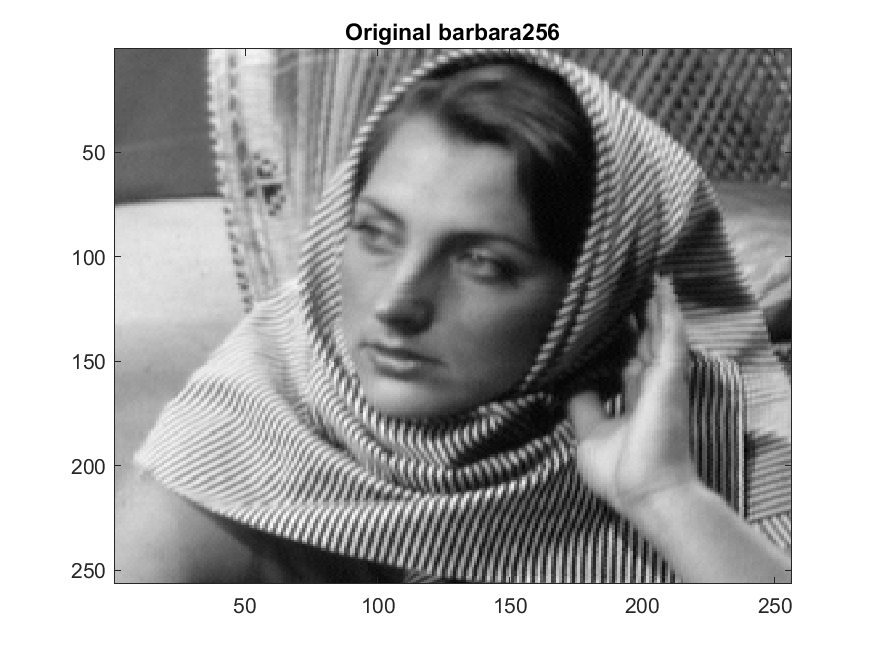
\includegraphics[width=\textwidth]{barbara256_orig.png}
        \caption{Original \texttt{barbara256}}
    \end{minipage}
    % \hfill
    \begin{minipage}[b]{0.45\textwidth}
        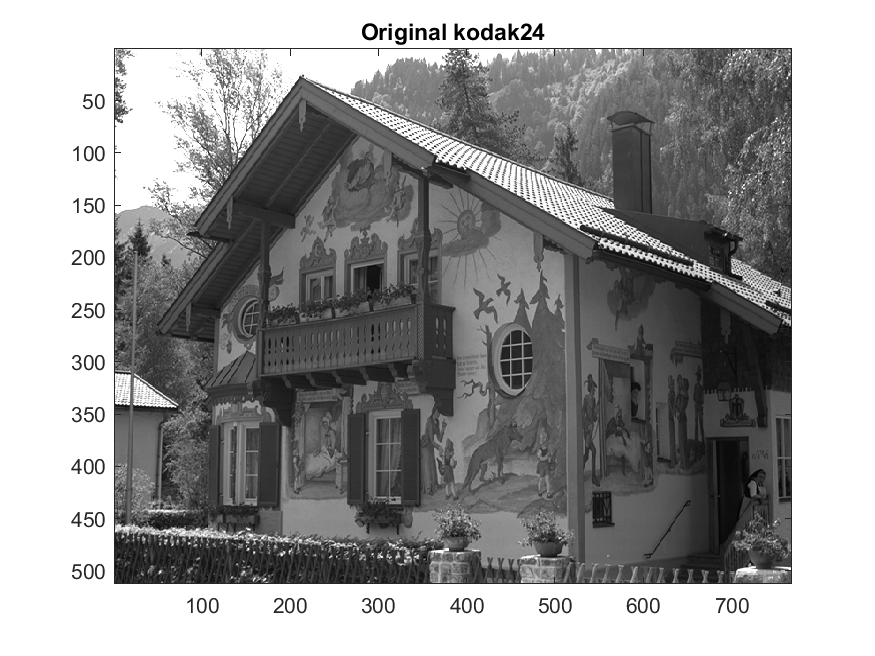
\includegraphics[width=\textwidth]{kodak24_orig.png}
        \caption{Original \texttt{kodak24}}
    \end{minipage}
    % \hfill
\end{figure}

\subsection*{(a)}

Adding a zero-mean gaussian noise with standard deviation of 5.

\begin{figure}[!htb]
    \centering
    \begin{minipage}[b]{0.45\textwidth}
        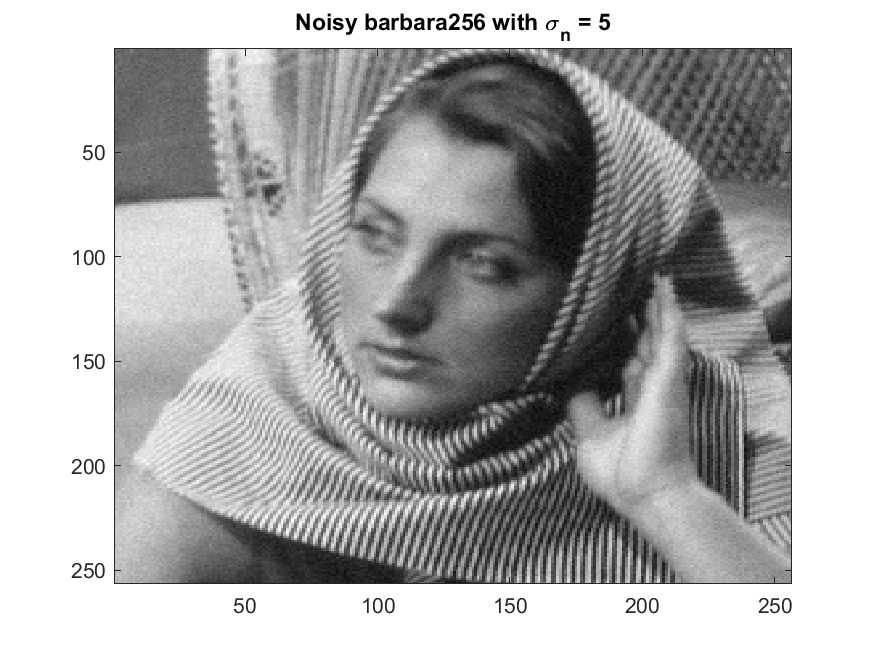
\includegraphics[width=\textwidth]{barbara256_noise5.png}
        % \caption{Noisy \texttt{barbara256}}
    \end{minipage}
    % \hfill
    \begin{minipage}[b]{0.45\textwidth}
        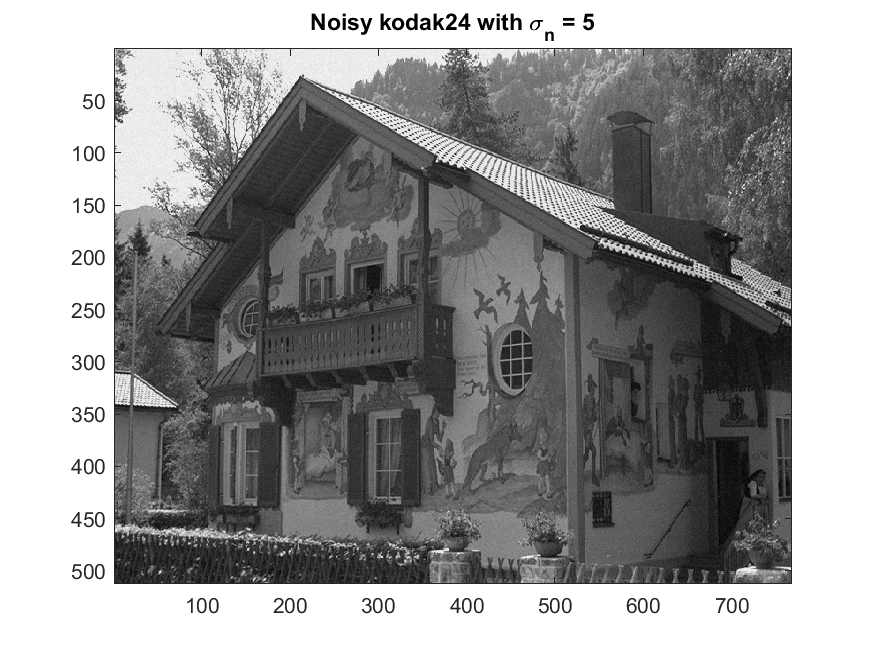
\includegraphics[width=\textwidth]{kodak24_noise5.png}
        % \caption{Noisy \texttt{kodak24}}
    \end{minipage}
\end{figure}

\begin{figure}[!htb]
    \centering
    \begin{minipage}[b]{0.3\textwidth}
        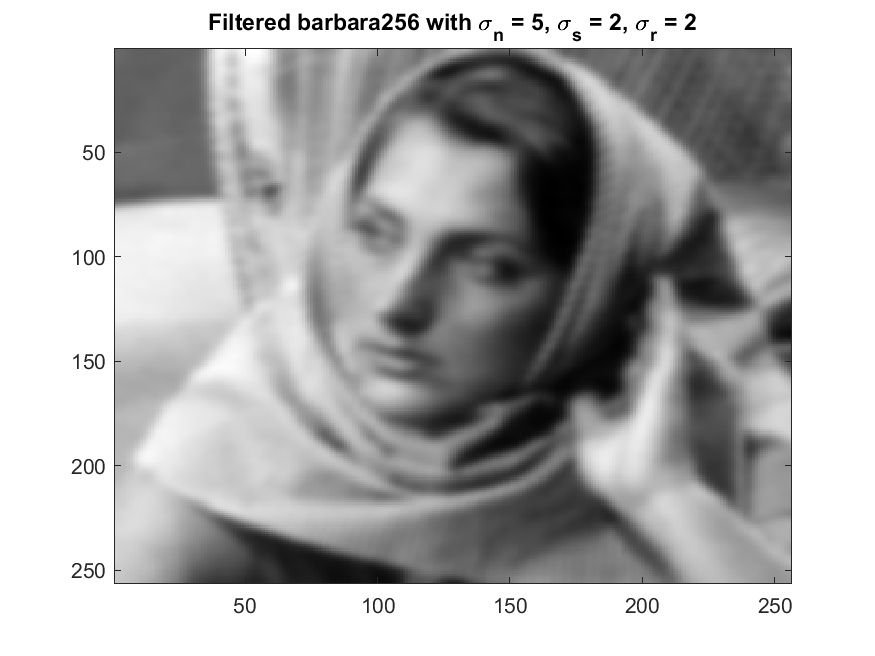
\includegraphics[width=\textwidth]{barbara256_5_2_2_5.png}
        % \caption{Noisy \texttt{barbara256}}
    \end{minipage}
    % \hfill
    \begin{minipage}[b]{0.3\textwidth}
        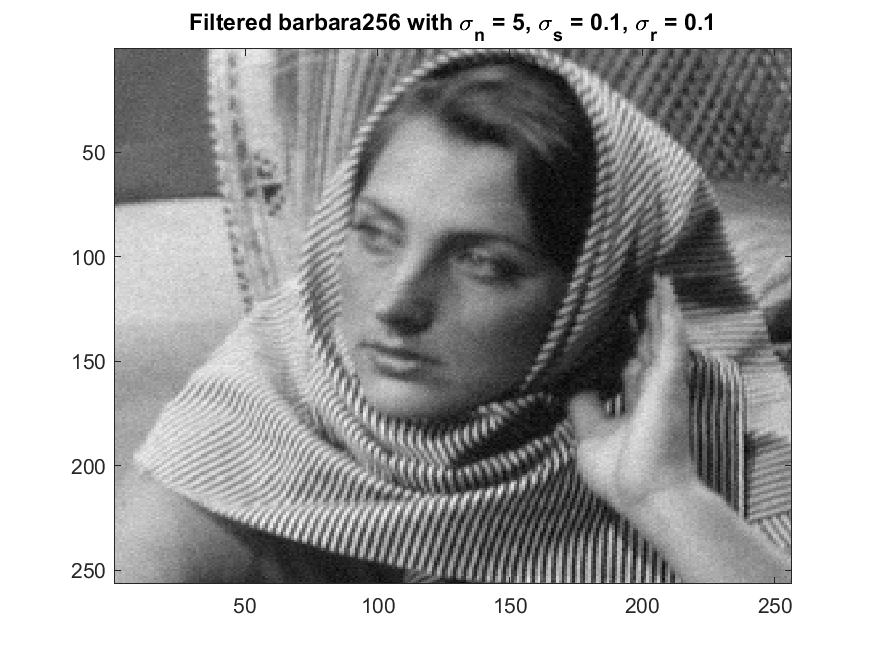
\includegraphics[width=\textwidth]{barbara256_5_0.1_0.1_7.png}
        % \caption{Noisy \texttt{kodak24}}
    \end{minipage}
    % \hfill
    \begin{minipage}[b]{0.3\textwidth}
        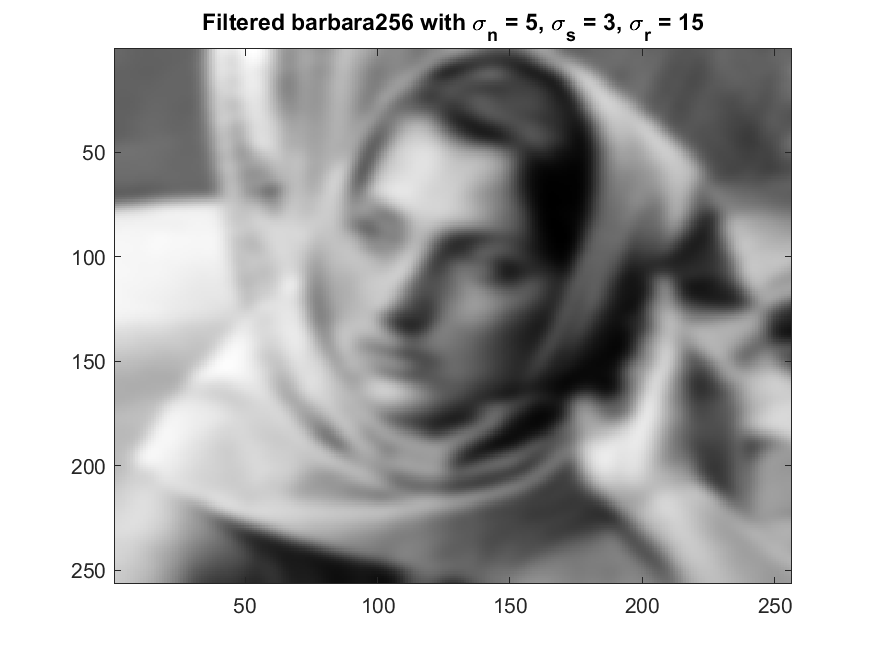
\includegraphics[width=\textwidth]{barbara256_5_3_15_9.png}
        % \caption{Noisy \texttt{kodak24}}
    \end{minipage}
\end{figure}

\begin{figure}[!htb]
    \centering
    \begin{minipage}[b]{0.3\textwidth}
        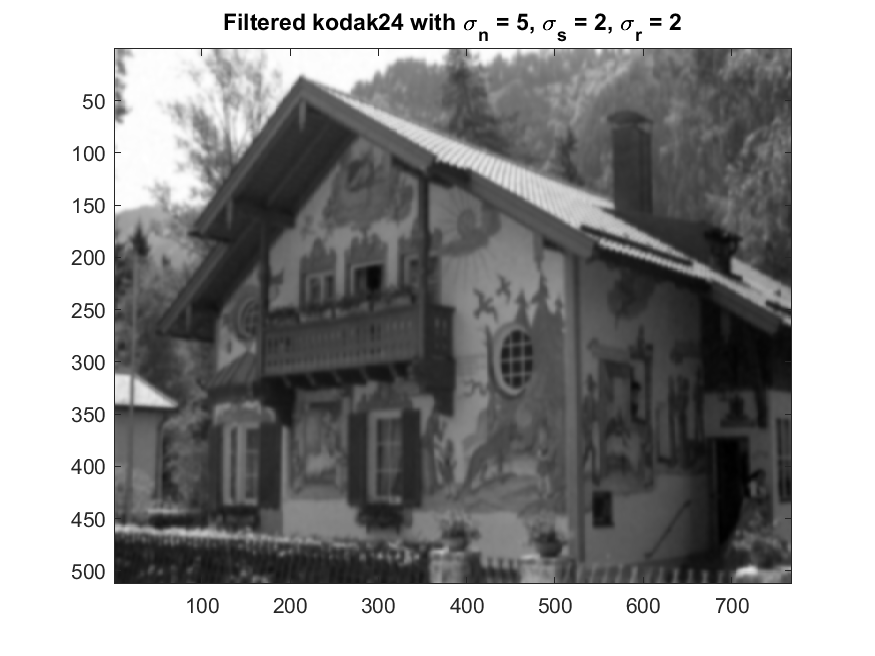
\includegraphics[width=\textwidth]{kodak24_5_2_2_6.png}
        % \caption{Noisy \texttt{barbara256}}
    \end{minipage}
    % \hfill
    \begin{minipage}[b]{0.3\textwidth}
        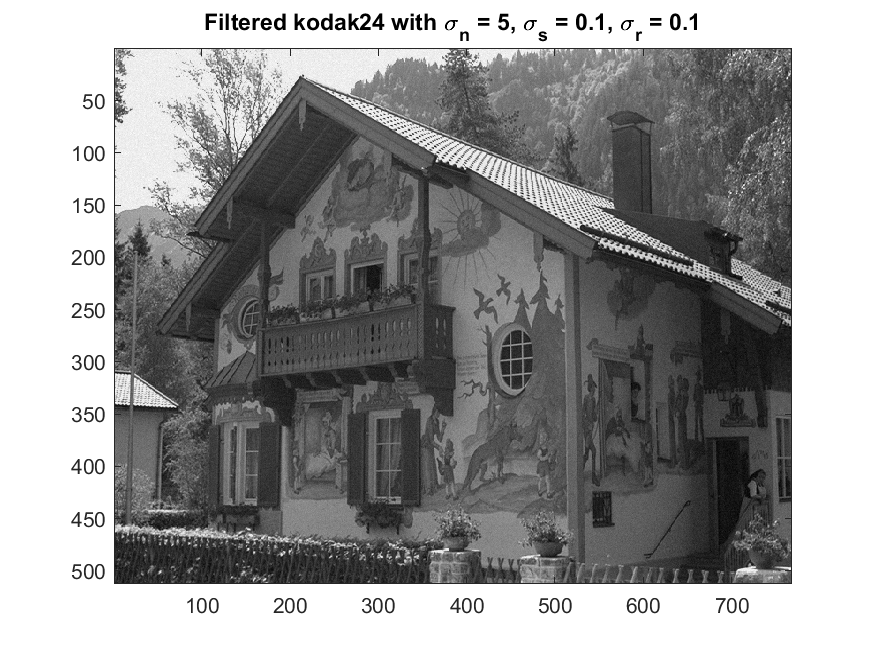
\includegraphics[width=\textwidth]{kodak24_5_0.1_0.1_8.png}
        % \caption{Noisy \texttt{kodak24}}
    \end{minipage}
    % \hfill
    \begin{minipage}[b]{0.3\textwidth}
        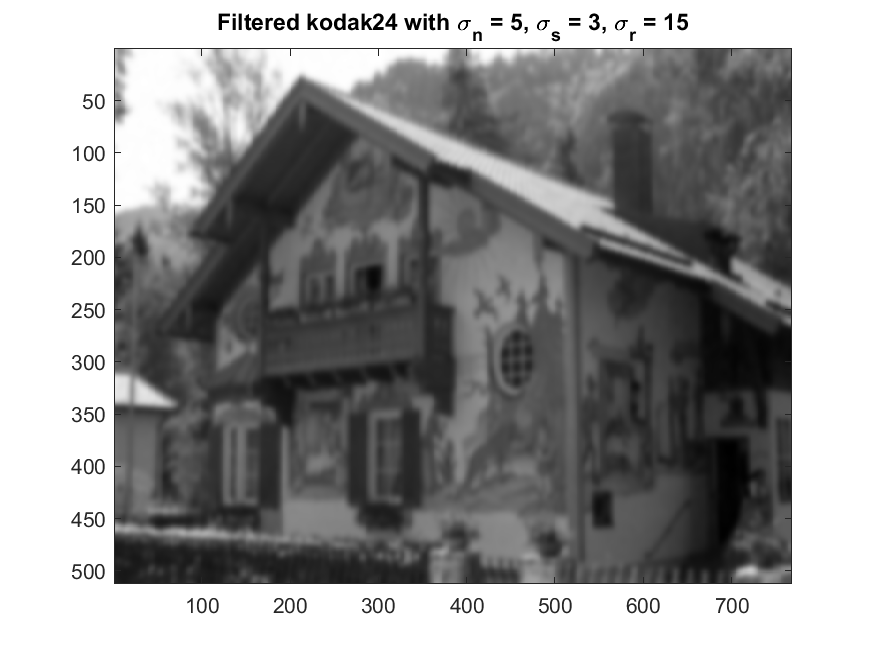
\includegraphics[width=\textwidth]{kodak24_5_3_15_10.png}
        % \caption{Noisy \texttt{kodak24}}
    \end{minipage}
\end{figure}

\newpage
As observed from the figures above, increasing the values of $\sigma_s$ and $\sigma_r$ results in greater blurring and noticeable smoothing of the images. 

This occurs because a larger number of neighboring pixels contribute significantly to the Gaussian filters, as the Gaussian distribution broadens with higher standard deviations. Also, the blurring effect is more pronounced when $\sigma_r$ is large, as it controls the degree to which pixels with varying intensities influence the average. While bilateral filtering does cause blurring, it still preserves the edges. This is evident in the Kodak images. Higher $\sigma_s$ and $\sigma_r$ values can enhance smoothing and noise reduction, but excessively high values may also result in the loss of fine details and sharpness.

\newpage
\subsection*{(b)}

Adding a zero-mean gaussian noise with standard deviation of 10.

\begin{figure}[!htb]
    \centering
    \begin{minipage}[b]{0.45\textwidth}
        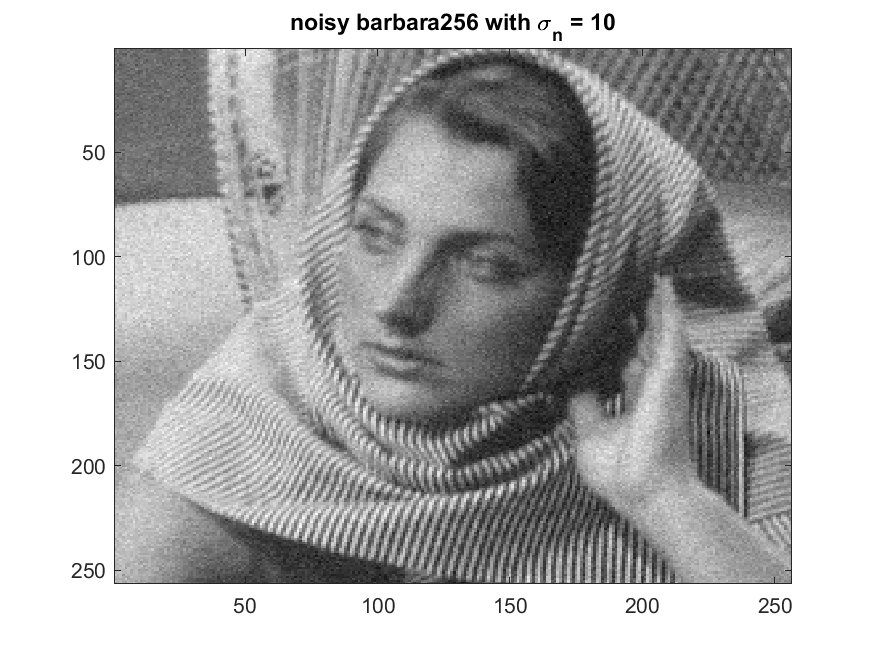
\includegraphics[width=\textwidth]{barbara256_noise10.png}
        % \caption{Noisy \texttt{barbara256}}
    \end{minipage}
    % \hfill
    \begin{minipage}[b]{0.45\textwidth}
        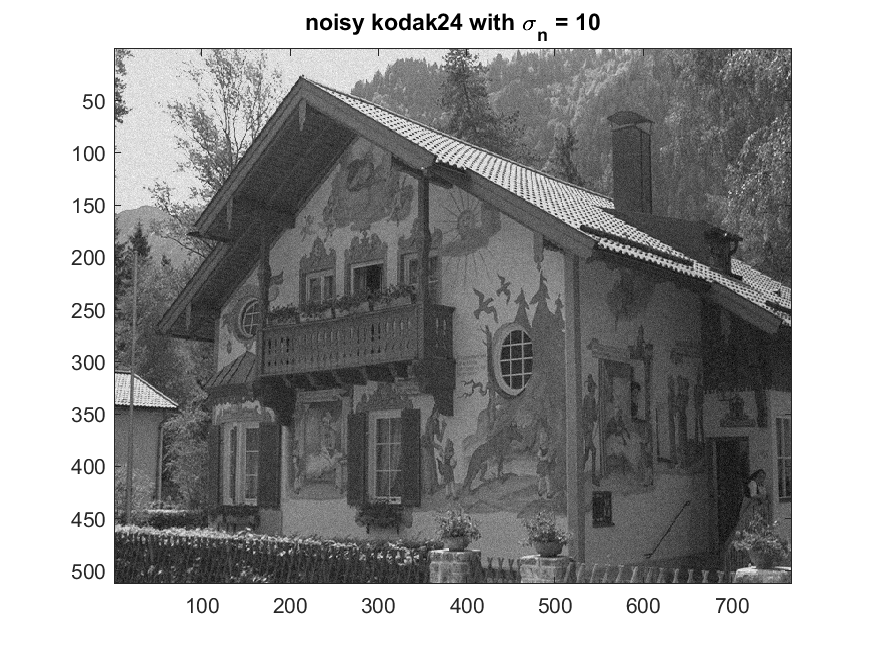
\includegraphics[width=\textwidth]{kodak24_noise10.png}
        % \caption{Noisy \texttt{kodak24}}
    \end{minipage}
\end{figure}

\begin{figure}[!htb]
    \centering
    \begin{minipage}[b]{0.3\textwidth}
        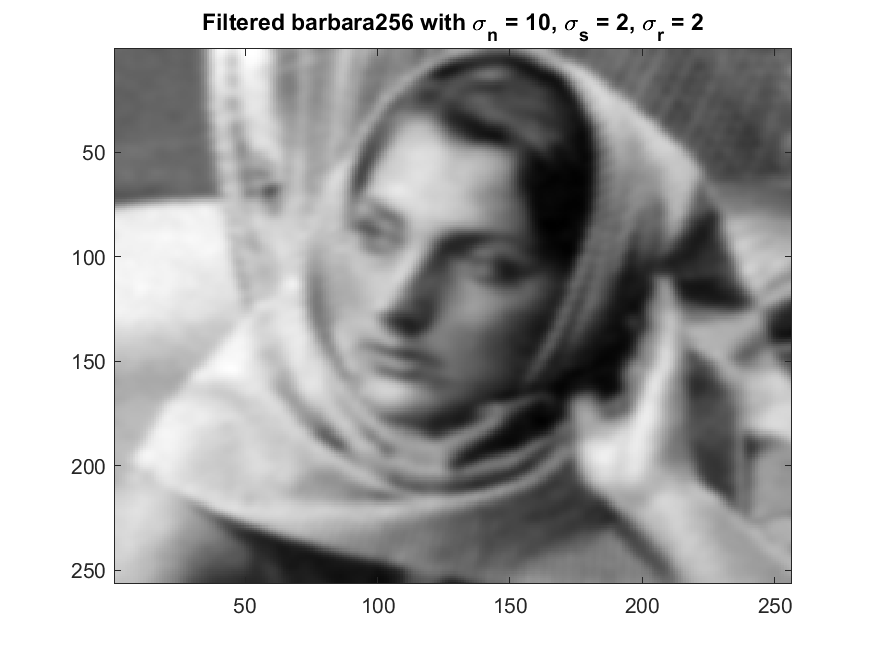
\includegraphics[width=\textwidth]{barbara256_10_2_2_13.png}
        % \caption{Noisy \texttt{barbara256}}
    \end{minipage}
    % \hfill
    \begin{minipage}[b]{0.3\textwidth}
        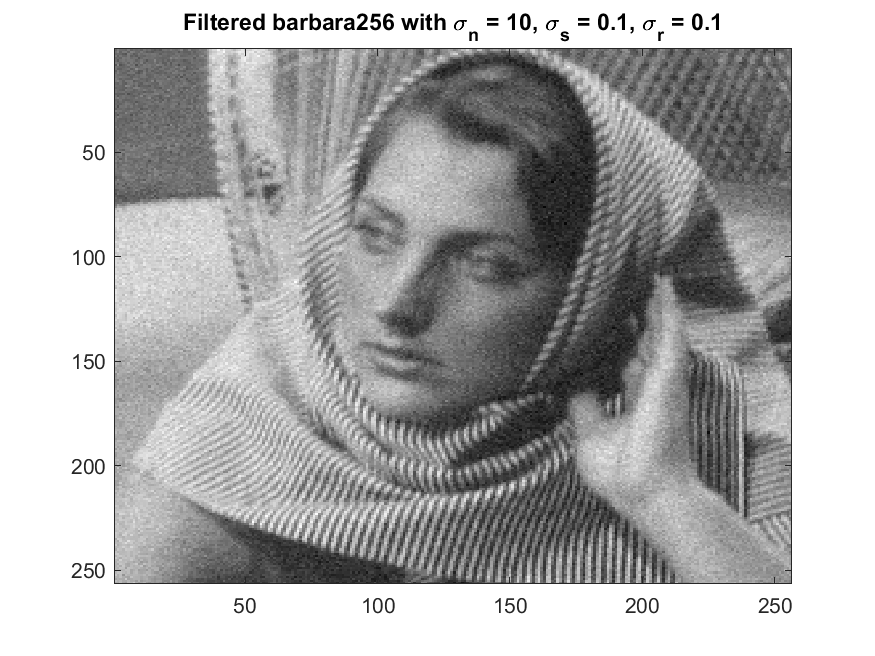
\includegraphics[width=\textwidth]{barbara256_10_0.1_0.1_15.png}
        % \caption{Noisy \texttt{kodak24}}
    \end{minipage}
    % \hfill
    \begin{minipage}[b]{0.3\textwidth}
        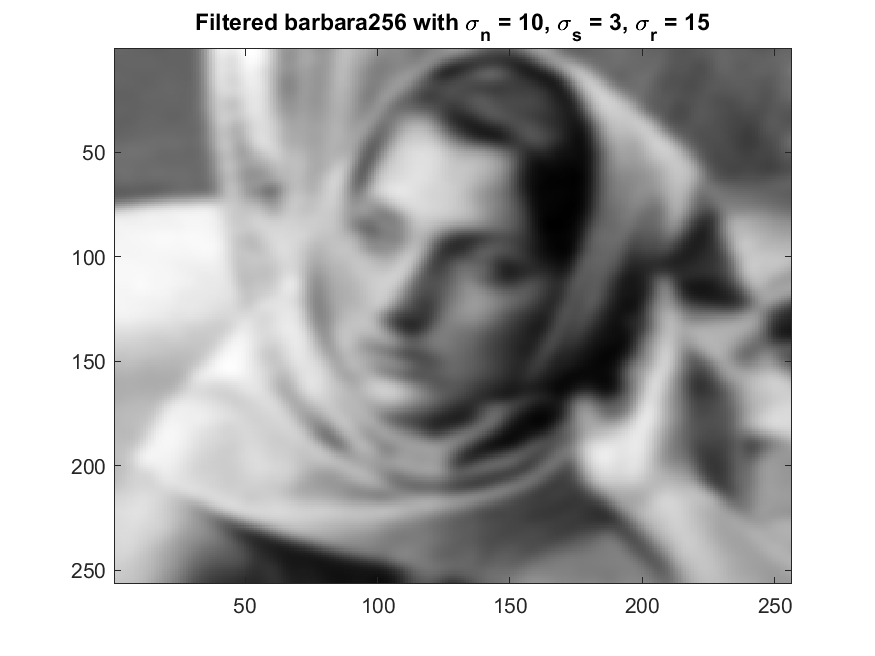
\includegraphics[width=\textwidth]{barbara256_10_3_15_17.png}
        % \caption{Noisy \texttt{kodak24}}
    \end{minipage}
\end{figure}

\begin{figure}[!htb]
    \centering
    \begin{minipage}[b]{0.3\textwidth}
        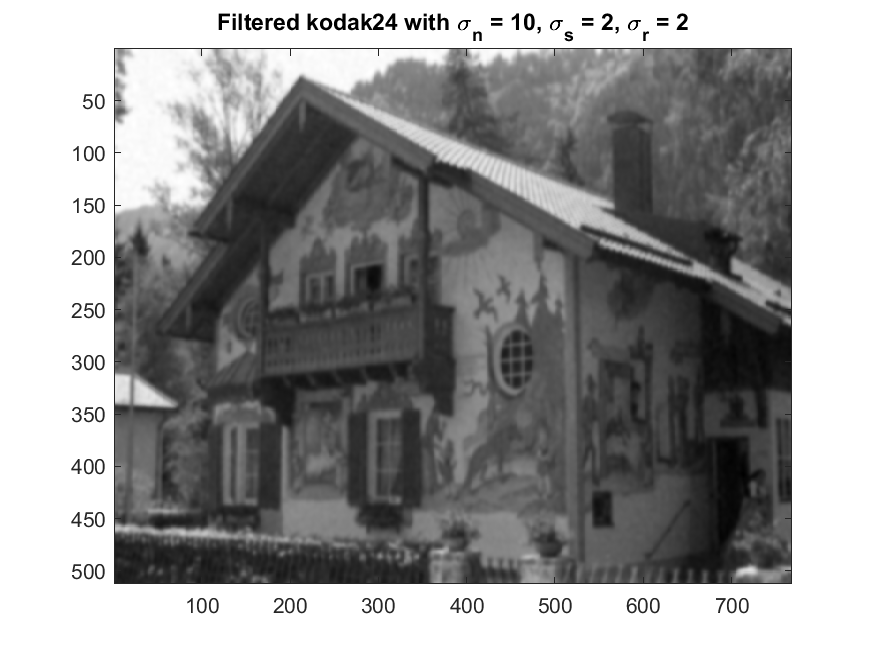
\includegraphics[width=\textwidth]{kodak24_10_2_2_14.png}
        % \caption{Noisy \texttt{barbara256}}
    \end{minipage}
    % \hfill
    \begin{minipage}[b]{0.3\textwidth}
        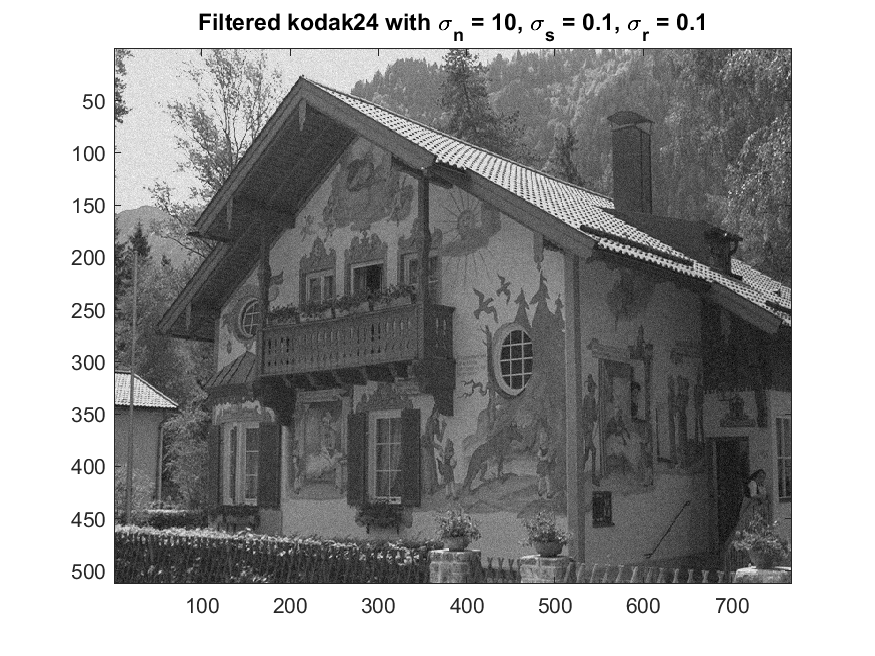
\includegraphics[width=\textwidth]{kodak24_10_0.1_0.1_16.png}
        % \caption{Noisy \texttt{kodak24}}
    \end{minipage}
    % \hfill
    \begin{minipage}[b]{0.3\textwidth}
        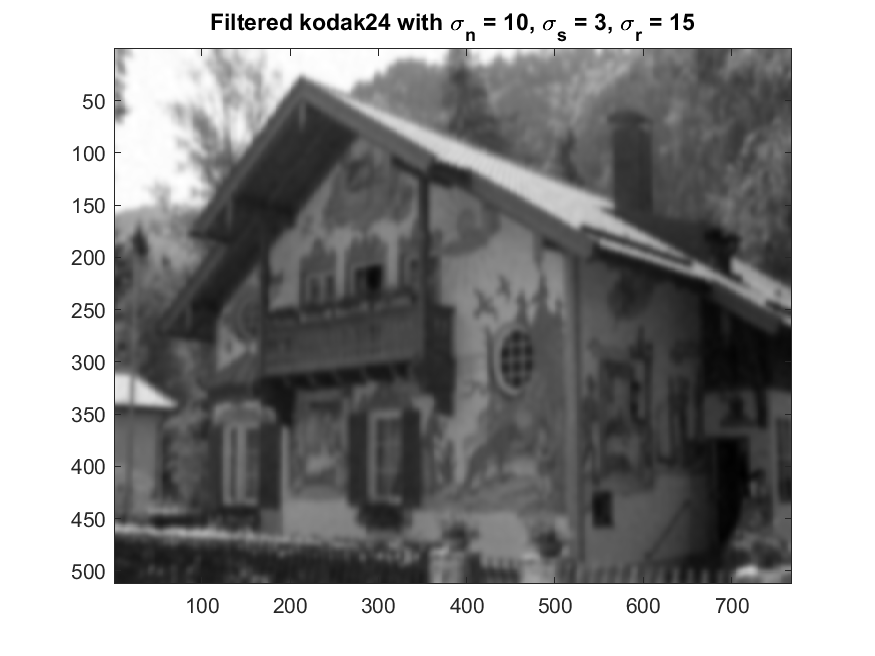
\includegraphics[width=\textwidth]{kodak24_10_3_15_18.png}
        % \caption{Noisy \texttt{kodak24}}
    \end{minipage}
\end{figure}

As we increase the standard deviation of gaussian noise, the intensities have more error now.

Hence we expect to see better filtering results, but low standard deviations doesn't
provide much smoothing to the noisy images, and hence is observed at the highest values.

\end{document}